%
% File: introduction.tex
% Author: Victor F. Brena-Medina
% Description: Introduction chapter where the biology goes.
%
\let\textcircled=\pgftextcircled
\chapter{Introduction}

\initial{T}his chapter will be used to acquaint the reader with the emerging UAV market, and the challenges it is facing on its way towards maturity.
Also, the reasons for its rapid evolution will be exposed and finally, focusing on the contents of this thesis, the personal motivation and the methodology will be explained to further expand on the topics of interest in the following chapters.

\section{Background information} \label{sec:background}

The first remotely radio controlled models appeared in the early twentieth century as small prototypes for potential manned aircraft. 
Afterwards, and during most of the century, the investigation and development lines were directed towards the military scope, in which the main objective of UAVs, which is still applied today, was to substitute manned aircraft in three types of military operations, commonly known as ``the three D's" \cite{daily2015,uasapplications2016}:

\begin{itemize}
	\item Dirty: operations performed in a contaminated environment.
	\item Dangerous: operations entailing some risk for the pilot.
	\item Dull: long and monotone operations, such as monitoring operations.
\end{itemize}

In the 70's and the 80's, efforts were directed to improve the technical characteristics of these vehicles.
But it was not until the late 80's when a revolution in the industry took place with the introduction of the GPS navigation system, whose accuracy in geolocation opened a whole new spectrum of possibilities.

Regarding the civil sector, the potential applications of UAVs in the non-military field are much more diverse.
Nowadays these vehicles are in the process of finding new niche positions in the civilian market, having been introduced up to now in different industry sectors such as agriculture, forest fire fighting, search and rescue, aerial photography, cartography, or security and surveillance, among others. 
Despite the latter, the use of UAVs for civil purposes is relatively recent in comparison with the military sector.
This late implementation in the civilian field was caused mainly by two limitations which are of minor relevance in the fighting industry: legislation and economy.
\cite{aguado2016}

\section{Socioeconomic environment}

Apart from ``the three D's'' mentioned in Section \ref{sec:background}, another reason for the embracement of UAVs within the industry shall be considered.
The final goal of any company is to create profit to their shareholders, which can be done either by increasing the revenues or by decreasing the costs of their activities.
UAVs enter in the latter category.
The consistent usage of smaller tools as compared with the manned workpower usually means that the equipment costs can be lowered, as well as the man-hours needed to perform the task \cite{airbusdemonstratesaircraftinspectionbydroneatfarnborough2016}, not to mention that most of the time the number of workers needed can be reduced to as low as one or two, in charge of operating the UAS (Unmanned Aerial System\footnote{UAS refers to the bigger system that incorporates one or more UAVs, as well as the Ground Control Station or other related subsystems}).

This phenomenon is already proving to be very effective for the companies taking advantage of it, but research also shows an even bigger potential that is still waiting to be exploited, claiming that UAVs could have replaced \$127 billion worth of human labour in 2015 \cite{wisniewski2016}, distributed in the sectors shown in Figure \ref{fig:pwc}.

\begin{figure}[htb]
	\centering
	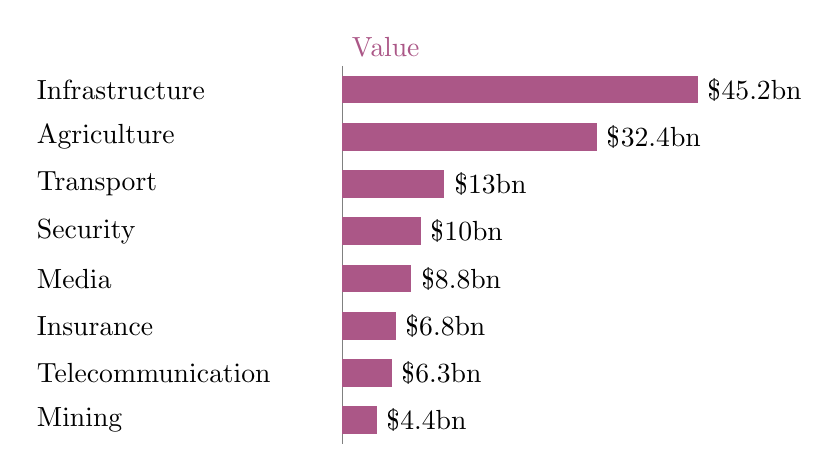
\begin{tikzpicture}

		\definecolor{purpleAtlas}{RGB}{171,87,135}

		%\draw[step=1cm,gray,very thin] (0,0) grid (10,6);

		\node[above right,purpleAtlas] at (4,6.1) {Value};
		\draw[black!50] (4,6.1) -- (4,1.3);
		\draw[purpleAtlas, line width=0.35cm] (4,5.8) -- (8.52,5.8);
			\node[right] at (0,5.8) {Infrastructure};
			\node[right] at (8.52,5.8) {\$45.2bn};
		\draw[purpleAtlas, line width=0.35cm] (4,5.2) -- (7.24,5.2);
			\node[right] at (0,5.2) {Agriculture};
			\node[right] at (7.24,5.2) {\$32.4bn};
		\draw[purpleAtlas, line width=0.35cm] (4,4.6) -- (5.3,4.6);
			\node[right] at (0,4.6) {Transport};
			\node[right] at (5.3,4.6) {\$13bn};
		\draw[purpleAtlas, line width=0.35cm] (4,4) -- (5,4);
			\node[right] at (0,4) {Security};
			\node[right] at (5,4) {\$10bn};
		\draw[purpleAtlas, line width=0.35cm] (4,3.4) -- (4.88,3.4);
			\node[right] at (0,3.4) {Media};
			\node[right] at (4.88,3.4) {\$8.8bn};
		\draw[purpleAtlas, line width=0.35cm] (4,2.8) -- (4.68,2.8);
			\node[right] at (0,2.8) {Insurance};
			\node[right] at (4.68,2.8) {\$6.8bn};
		\draw[purpleAtlas, line width=0.35cm] (4,2.2) -- (4.63,2.2);
			\node[right] at (0,2.2) {Telecommunication};
			\node[right] at (4.63,2.2) {\$6.3bn};
		\draw[purpleAtlas, line width=0.35cm] (4,1.6) -- (4.44,1.6);
			\node[right] at (0,1.6) {Mining};
			\node[right] at (4.44,1.6) {\$4.4bn};

	\end{tikzpicture}
	\caption{Distribution of potential UAV markets \cite{wisniewski2016}}
	\label{fig:pwc}
\end{figure}


\section{Legal framework}

\cite{manualonremotelypilotedaircraftsystemsrpas2015,ley182014de15deoctubredeaprobaciondemedidasurgentesparaelcrecimientolacompetitividadylaeficiencia2014}

\section{Motivation}

Traditionally, the most important payload that could be carried in an aircraft was human beings, that would perform their mission while aloft.
Nevertheless, the advancements on sensing technology and wireless communications have forced a change on traditional aviation.
Apart from commercial aviation, where the final objective is to transport people form one place to another, in almost any other mission the role of the human workforce is to pilot the aircraft and/or operate the payload systems.
This secondary role of the human operators implies that, given the maturity of the involved technology, they could be substituted by intelligent computer systems or, at least, disembarked form the aircraft into a safer Ground Control Station (GCS).
The process of ``unmanning'' the aircraft also brings the advantages of decreasing the weight of the aircraft and thus improving its endurance and manoeuvrability, avoids putting the pilot in a dangerous situation, and helps alleviate the errors associated with tedious and repetitive tasks, among others.

However, there are also some downsides.
The most accused ones for experienced pilots are those related with the loss of situational awareness that comes as a result of eliminating the physical cues (body inertia, vibrations\ldots) and relying on instrumental readings only, and also the limited number of control input, which for civil UAVs do not exceed 8 or 9 scalar channels.
Thus, for the effective incorporation of Unmanned Vehicles into professional activities it is required to extend and automate some of the tasks that are traditionally performed by the onboard pilot.

Finally, for this project, the goal is to provide a system that reduces the possibility of it crashing with nearby obstacles, so that regular operations are carried with a higher level of safety.
Eventually, the authorities will consider this increase in overall safety causing the modification of existing regulations to a more permissive set, allowing the industry to take advantage of all the benefits that the incorporation of UAVs could bring to their activities.

\section{Project objectives}

\section{Methodology}

\section{Time planning}

